\section{ \bfseries Quadratic Program (QP)}
The quadratic program (QP) is considered in the form (assume that $A$ has full column rank)\\
\begin{align*}
&\min_{x} \quad \phi=\frac{1}{2} x^{\prime} H x+g^{\prime} x \tag{2}\label{con:op2}\\
& s.t. \quad A^{\prime} x=b\\
& \quad \quad  l\le x \le u
\end{align*}
%%%%%%%%%%%%%%%%%%%%%%%%%%%%%%%%%%%%%%%%%%
%%%%%%%%%%%%%%%%%%%%%%%%%%%%%%%%%%%%%%%%%%%%%%%%%%%%%%%%%%%%%%%%%%%%%%%%%%%%%%%%%%%%%
%%%%%%%%%%%%%%%%%%%%%%%%%%%%%%%%%%%%%%%%%%%
%%%%%%%%%%%%%%%%%%%%%%%%%%%%%%%%%%%%%%%%%%
%%%%%%%%%%%%%%%%%%%%%%%%%%%%%%%%%%%%%%%%%%%
\subsection{\bfseries Lagrangian function}
\begin{shaded}
{ Question: What is the Lagrangian function for this problem?}
\end{shaded}
The quadratic program problem (\ref{con:op2}) can be equivalent to the inequailty constrained form
\begin{align*}
&\min_{x} \quad \phi=\frac{1}{2} x^{\prime} H x+g^{\prime} x \tag{2.1}\label{con:op2.1}\\
& s.t. \quad A^{\prime} x=b\\
& \quad \quad  c(x)=\begin{bmatrix}
x-l \\ u-x\end{bmatrix}=\left[I\quad -I\right]^{\prime}x+\begin{bmatrix}
-l \\ u\end{bmatrix}\ge 0\Leftrightarrow C^{\prime}x \ge d
\end{align*}
Lagrangian function\\
$$L(x,y,z)=\frac{1}{2}x^{\prime}Hx+g^{\prime}x-y^{\prime}\left(A^{\prime}x-b\right)-z^{\prime}\left(C^{\prime}x-d\right)\eqno{(2.2)}$$
%%%%%%%%%%%%%%%%%%%%%%%%%%%%%%%%%%%%%%%%%%
%%%%%%%%%%%%%%%%%%%%%%%%%%%%%%%%%%%%%%%%%%%
%%%%%%%%%%%%%%%%%%%%%%%%%%%%%%%%%%%%%%%%%%
%%%%%%%%%%%%%%%%%%%%%%%%%%%%%%%%%%%%%%%%%%%
%%%%%%%%%%%%%%%%%%%%%%%%%%%%%%%%%%%%%%%%%%
%%%%%%%%%%%%%%%%%%%%%%%%%%%%%%%%%%%%%%%%%%%
\subsection{\bfseries Optimality conditions}
\begin{shaded}
{Question: Write the nesessary and sufficient optimality conditions for this problem.}
\end{shaded}
\begin{align*}
& \nabla_{x} L\left(x,y,z\right)=Hx+g-Ay-Cz=0\tag{2.3}\\
& \nabla_{y} L\left(x,y,z\right)=-\left(A^{\prime}x-b\right)=0\tag{2.4}\\
& \nabla_{z} L\left(x,y,z\right)=-\left(C^{\prime}x-d\right) \le 0\tag{2.5}\\
& z \ge 0 \tag{2.6}\\
& \left(C^{\prime}x-d\right)_iz_i=0 \quad i=1,2,...,m_c \tag{2.7}
\end{align*}
%%%%%%%%%%%%%%%%%%%%%%%%%%%%%%%%%%%%%%%%%%
%%%%%%%%%%%%%%%%%%%%%%%%%%%%%%%%%%%%%%%%%%%
%%%%%%%%%%%%%%%%%%%%%%%%%%%%%%%%%%%%%%%%%%
%%%%%%%%%%%%%%%%%%%%%%%%%%%%%%%%%%%%%%%%%%%
%%%%%%%%%%%%%%%%%%%%%%%%%%%%%%%%%%%%%%%%%%
%%%%%%%%%%%%%%%%%%%%%%%%%%%%%%%%%%%%%%%%%%%
\subsection{\bfseries Primal-dual interior-point algorithm}
\begin{shaded}
{Question: Write pseudo-code for a primal-dual interior-point algorithm for solution of this
problem. Explain each major step in your algorithm.}
\end{shaded}
{\setmainfont{Times New Roman}\bfseries Pseudo-code}
\begin{algorithm}[!h]
	\caption{Primal-Dual Predictor-Corrector Interior-Point Algorithm}
	\begin{algorithmic}[1]
	    \STATE Given an input $H$, $g$, $A$, $b$, $C$, $d$ and compute the starting point $x_0$, $y_0$, $z_0$, $s_0$ with ($z_0$,$s_0$)>0\\
		\STATE Compute the residuals $r_L$, $r_A$, $r_C$, $r_{sz}$ and duailty gap $\mu$\\
		\STATE Check convergence conditions\\
		
        \WHILE {(not converged)}\\
		\STATE Compute the affine step direction $\Delta x^{aff}$, $\Delta z^{aff}$ and $\Delta s^{aff}$\\
		\STATE Compute the affine step size $\alpha ^{aff}$\\
		\STATE Compute the affine duality gap $\mu ^{aff} $\\
		\STATE Compute centering parameter $\sigma$\\
		\STATE Compute affine-centering-correction direction\\
		\STATE Compute the step size $\alpha * \eta$ and update the iteration of $x$, $y$, $z$ and $s$ to take the actual step\\
		\STATE Re-compute the residuals $r_L$, $r_A$, $r_C$, $r_{sz}$ and duailty gap $\mu$\\
		\STATE Check convergence conditions and stop if it converged\\
		\ENDWHILE
    \end{algorithmic}
\end{algorithm}

The inequality in the form of this problem requires further introduction of slack variables
$$s \triangleq C^{\prime} x-d \ge 0\eqno{(2.8)}$$
implies
\begin{align*}
& -C^{\prime}x+s+d=0\tag{2.9}\\
& s \ge 0
\end{align*}
The optimality conditions can be expressed as
\begin{align*}
& r_L=Hx+g-Ay-Cz=0\tag{2.10}\\
& r_A=-\left(A^{\prime}x-b\right)=0\tag{2.11}\\
& r_C=-\left(C^{\prime}x-d\right) \ge 0\tag{2.12}\\
& r_{SZ}=SZe=0\tag{2.13}\\
& s \ge 0, \quad z \ge 0\tag{2.14}
\end{align*}

Several enhancements have a significant effect on practical performance, so the Primal-dual interior-point algorithm implemented here is based on Mehrotra's predictor-corrector method. \\[0.3cm]
In the first step, a set of feasible starting point needs to be computed. A heuristic\cite{NoceWrig06} for starting point on p.484 in Nocedal \& Wright is introduced.
\begin{algorithm}[H]
	\caption{Heuristic for an starting point}
	\begin{algorithmic}[1]
	    \STATE Given an input $\bar{x}$, $\bar{y}$, $\bar{z}$, $\bar{s}$ with ($\bar{z}$,$\bar{s}$)>0\\
		\STATE Compute the residuals $r_L$, $r_A$, $r_C$ and  $r_{sz}$\\
		\STATE Compute affine search direction from $\bar{x}$, $\bar{y}$, $\bar{z}$ and $\bar{s}$\\
		\STATE $x=\bar{x}$, $y=\bar{y}$, $z=max\{1,|\bar{z}+\Delta z^{aff}|\}$, $s=max\{1,|\bar{s}+\Delta s^{aff}|\}$
    \end{algorithmic}
\end{algorithm}
The Primal-dual interior-point algorithm is based on iterative calculation. And the strict positivity of $z$ and $s$ is maintained throughout and each step is a Newton-like step involving a centering component. Therefore, in fact, the Primal-dual interior-point algorithm uses a less aggressive Newton direction, which is to control the iteration point so that it gradually approaches the constraint boundary and the optimal solution. The specific method is that when the Newton method is used to solve a nonlinear system, it is not required to directly achieve $r_{SZ}=SZe=0$ in each iteration, but to make it equal to a gradually decreasing value, which is $r_{SZ}=SZe=\sigma \mu e$, where $\mu$ is the current duailty gap, and $\sigma \in [0,1]$ is the center parameter used to control the descent speed.\\
The specific steps of iteration are: An affine step is computed. 
$$\left[\begin{array}{cccc}
H & -A & -C & 0 \\
-A^{\prime} & 0 & 0 & 0 \\
-C^{\prime} & 0 & 0 & I \\
0 & 0 & S & Z
\end{array}\right]\left[\begin{array}{l}
\Delta x^{a f f} \\
\Delta y^{a f f} \\
\Delta z^{a f f} \\
\Delta s^{a f f}
\end{array}\right]=\left[\begin{array}{c}
-r_{L} \\
-r_{A} \\
-r_{C} \\
-r_{S Z}
\end{array}\right]\eqno{(2.15)}$$
Then the center parameter $\sigma$ will be made small if the affine step is good, or to be set as 1 if the affine step is bad, by which the iteration point can stay close to central path. So $\alpha^{aff}$ is defined as the largest value satisfying
\begin{align*}
&z+\alpha^{a f f} \Delta z^{a f f} \geq 0\tag{2.16}\\
&s+\alpha^{a f f} \Delta s^{a f f} \geq 0\tag{2.17}
\end{align*}
Then Duality gap $\mu_{aff}$ is defined for affine step
$$\mu^{a f f}=\frac{\left(z+\alpha^{a f f} \Delta z^{a f f}\right)^{\prime}\left(s+\alpha^{a f f} s^{a f f}\right)}{m_{c}}\eqno{(2.18)}$$
The centering parameter is calculated as a heuristic
$$\sigma=\left(\frac{\mu^{a f f}}{\mu}\right)^{3} \quad with \quad \mu=\frac{z^{\prime} s}{m_{c}}\eqno{(2.19)}$$
Then affine-centering-correction direction is computed by solving
$$\left[\begin{array}{cccc}
H & -A & -C & 0 \\
-A^{\prime} & 0 & 0 & 0 \\
-C^{\prime} & 0 & 0 & I \\
0 & 0 & S & Z
\end{array}\right]\left[\begin{array}{c}
\Delta x \\
\Delta y \\
\Delta z \\
\Delta s
\end{array}\right]=-\left[\begin{array}{c}
r_{L} \\
r_{A} \\
r_{C} \\
r_{S Z}+\Delta S^{a f f} \Delta Z^{a f f} e-\sigma \mu e
\end{array}\right]\eqno{(2.20)}$$
Update
$$\left[\begin{array}{l}
x \\
y \\
z \\
s
\end{array}\right]=\left[\begin{array}{l}
x+\eta \alpha \Delta x \\
y+\eta \alpha \Delta y \\
z+\eta \alpha \Delta z \\
s+\eta \alpha \Delta s
\end{array}\right]\eqno{(2.21)}$$
Finally the residuals are recomputed and convergence is defined as situation that the residuals $r_L$, $r_A$, $r_C$ and  $r_{SZ}$ are all below a given small value $\epsilon$.
%%%%%%%%%%%%%%%%%%%%%%%%%%%%%%%%%%%%%%%%%%
%%%%%%%%%%%%%%%%%%%%%%%%%%%%%%%%%%%%%%%%%%%
%%%%%%%%%%%%%%%%%%%%%%%%%%%%%%%%%%%%%%%%%%
%%%%%%%%%%%%%%%%%%%%%%%%%%%%%%%%%%%%%%%%%%%
%%%%%%%%%%%%%%%%%%%%%%%%%%%%%%%%%%%%%%%%%%
%%%%%%%%%%%%%%%%%%%%%%%%%%%%%%%%%%%%%%%%%%%
\newpage
\subsection{\bfseries Primal-dual interior-point algorithm implementation}
\begin{shaded}
{Question: Implement the primal-dual interior-point algorithm and test it. You must provide commented code as well as driver files to test your code, documentation that it works, and performance statistics.}
\end{shaded}
The matlab code of Primal-dual interior-point algorithm is showed here\\

{\setmainfont{Courier New Bold} \scriptsize            
\begin{lstlisting}
function [x,output]=PD_ipQP(H,g,A,b,C,d,x0,y0,z0,s0)
% PD_ipQP   Primal-dual interior-point algorithm
%
%          min  0.5*x'*H*x+g'*x
%           x
%          s.t. A x  = b      
%               C x >= d      
%         rL = Hx + g − Ay − Cz = 0 
%         rA = −Ax + b = 0 (Lagrange multiplier y)
%         rC = −Cx + s + d = 0 (Lagrange multiplier z)
%         s ≥ 0 (Slack variables )
%         sz = 0
% Syntax: [x,output]=PD_ipQP(H,g,A,b,C,d,x0,y0,z0,s0)
%         output.fval: minimum value
%         output.y: final y
%         output.s: final s
%         output.z: final z
%         output.Xarray: Iteration trajectory  
          
iteration_max=50;
epsilon=1.0e-9;
eta=0.995;
noeq=0;
Xarray=[];
Xarray=[Xarray x0];
nh=size(H,1);%dimension of x
na=size(A,2);%A'x=b
nc=size(C,2);%C'x>=d
e=ones(nc,1);
%residual
S0=diag(s0);
Z0=diag(z0);
%if no equlity equations
if isempty(A)&isempty(b)
    noeq=1;
end

if  noeq==1
    rL=H*x0+g-C*z0;
    rA=0.*x0;
    rC=s0+d-C'*x0;
    rsz=S0*Z0*e;
else
    rL=H*x0+g-A*y0-C*z0;
    rA=b-A'*x0;
    rC=s0+d-C'*x0;
    rsz=S0*Z0*e;
end

%duality gap
mu=(z0'*s0)/nc;

stop_flag=0;
iteration=0;
x=x0;
y=y0;
S=S0;
Z=Z0;
while(~stop_flag&iteration<=iteration_max)
    
    H_bar=H+C*(inv(S)*Z)*C';
    if noeq==1
     KKT=H_bar;
    else
    KKT=[H_bar -A;-A' zeros(na,na)];
    end
    
    [L, D, p] = ldl(KKT, 'lower', 'vector');
    %Affine Direction
    rL_bar=rL-C*(inv(S)*Z)*(rC-inv(Z)*rsz);
    if noeq==1
        KKT_b=-rL_bar;
    else
    KKT_b=-[rL_bar;rA];
    end
    delta_xy=zeros(size(KKT_b,1),1);
    delta_xy(p) = L'\(D\(L\KKT_b(p)));
    delta_x=delta_xy(1:nh);
    delta_z=-(inv(S)*Z)*C'*delta_x+(inv(S)*Z)*(rC-inv(Z)*rsz);
    delta_s=-inv(Z)*rsz-inv(Z)*S*delta_z;
    
    %compute the lagest alf
    z=diag(Z);
    s=diag(S);
    delta_zs=[delta_z;delta_s];
    alf_c=-[z;s]./delta_zs;
    alf_aff=min([1;alf_c(delta_zs<0)]);
    
    %compute the affine duality gap
    mu_aff=(z+alf_aff*delta_z)'*(s+alf_aff*delta_s)/nc;
    %compute the centering parameter
    sigma=(mu_aff/mu)^3;
    
    %Affine-Centering-Correction Direction
    delta_S=diag(delta_s);
    delta_Z=diag(delta_z);
    rsz_bar=rsz+delta_S*delta_Z*e-sigma*mu*e;
    %update Affine Direction
    rL_bar=rL-C*(inv(S)*Z)*(rC-inv(Z)*rsz_bar);
    if noeq==1
        KKT_b=-rL_bar;
    else
    KKT_b=-[rL_bar;rA];
    end
    delta_xy=zeros(size(KKT_b,1),1);
    delta_xy(p) = L'\(D\(L\KKT_b(p)));
    delta_x=delta_xy(1:nh);
    delta_y=delta_xy(nh+1:end);
    delta_z=-(inv(S)*Z)*C'*delta_x+(inv(S)*Z)*(rC-inv(Z)*rsz_bar);
    delta_s=-inv(Z)*rsz_bar-inv(Z)*S*delta_z;
    %update alf
    delta_zs=[delta_z;delta_s];
    alf_c=-[z;s]./delta_zs;
    alf_aff=min([1;alf_c(delta_zs<0)]);
    alf_bar=alf_aff*eta;
    %compute new state
    x=x+alf_bar*delta_x;
    y=y+alf_bar*delta_y;
    z=z+alf_bar*delta_z;
    s=s+alf_bar*delta_s;
    Z=diag(z);
    S=diag(s);
    %compute residuals
    if noeq==1
        rL=H*x+g-C*z;
        rA=0.*x;
        rC=s+d-C'*x;
        rsz=S*Z*e;
    else
        rL=H*x+g-A*y-C*z;
        rA=b-A'*x;
        rC=s+d-C'*x;
        rsz=S*Z*e;
    end
    mu=z'*s/nc;
    %stop judge
    judge = [norm(rL,1), norm(rA,1), norm(rC,1), abs(mu)];
    stop_flag = (length(judge(judge < epsilon)) == 4);
    Xarray=[Xarray x];
    iteration=iteration+1;
end
fval=0.5*x'*H*x+g'*x;
output.fval=fval;
output.y=y;
output.s=s;
output.z=z;
output.Xarray=Xarray;
output.iteration=iteration;
end
\end{lstlisting}}

In the later section on the comparison of the two algorithms, the test of the algorithm with a test problem that can be randomly generated and control the size of the variable is carried out. Here is just a simple verification of the feasibility of the algorithm.\\
Two problems that meet the format requirements are used to test the implemented algorithm, a quadratic programming problem with equality constraints and a quadratic programming problem with only inequality constraints($A=0, b=0$)\\
\begin{align*}
    &\min_{x}\quad \phi(x)=\left(x_1-1\right)^2+\left(x_2-2.5\right)^2 \tag{2.22}\\
    &\text{s.t.} \quad x_1-x_2= 1   \qquad \qquad -1<x_1<2\\
    &\quad \quad -1<x_1<2 \qquad \qquad -1<x_2<2\\
    &\quad \quad -1<x_2<2\\
    &\quad \qquad \text{problem1} \qquad \qquad \qquad \text{problem2}
\end{align*}\\
Four starting points are chose to check the result of the problem1 and problem2 respectively, $A(-1,4)$ and $B(4,-1)$ which located outside the feasible area, $C(1,-1)$ which located at the edge of the inequailty constraint, and $D(0,0)$ which located inside the feasible area. First $H$ and $g$ of the objective function which will be used in the test are calculated
$$H=\begin{bmatrix}
2&0\\
0&2
\end{bmatrix} \qquad 
g=\begin{bmatrix}
-2\\
-5
\end{bmatrix}$$
The driver files are stated in the appendix \ref{6.2.1} and \ref{6.2.2}. The iterative trajectory in the contour for the problem1 is showed here
\vspace{-0.3cm}
\begin{figure}[H]
\centering
\setlength{\abovecaptionskip}{-0.2cm} 
\setlength{\belowcaptionskip}{-0.5cm} 
\subfigure[$A(-1,4)$]{
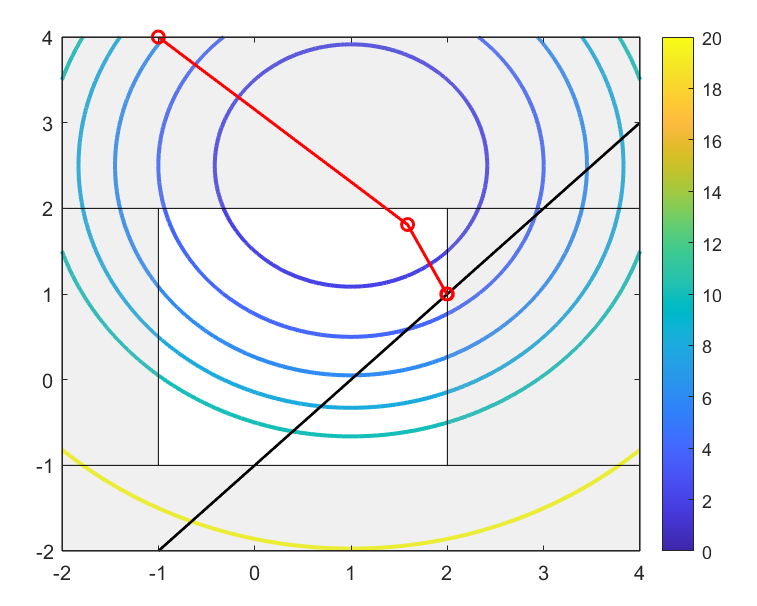
\includegraphics[scale=0.35]{figures/QP_IP_1_A.PNG}
%\caption{fig1}
}
\quad
\subfigure[$B(4,-1)$]{
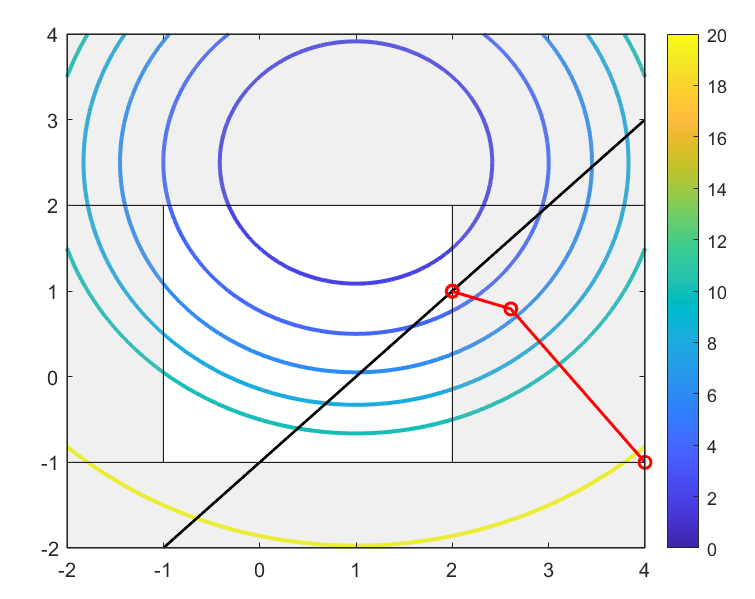
\includegraphics[scale=0.35]{figures/QP_IP_1_B.PNG}
}
\quad
\subfigure[$C(1,-1)$]{
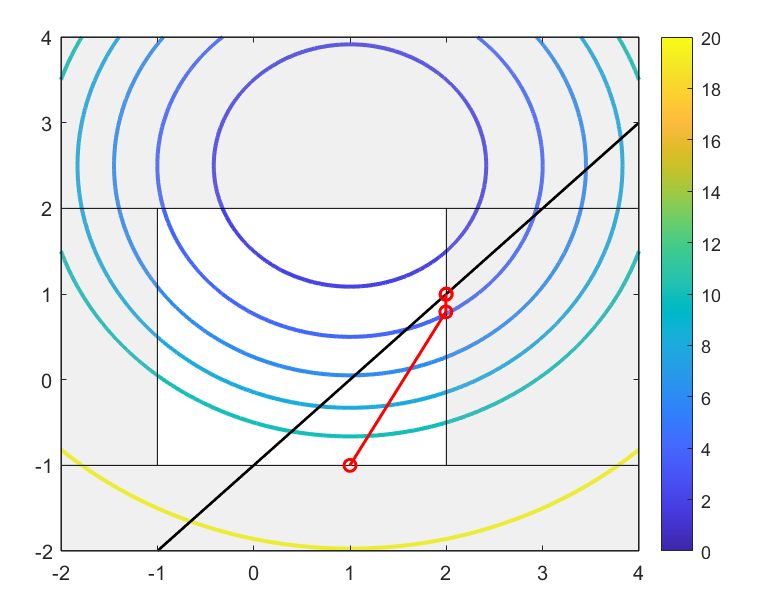
\includegraphics[scale=0.35]{figures/QP_IP_1_C.PNG}
}
\quad
\subfigure[$D(0,0)$]{
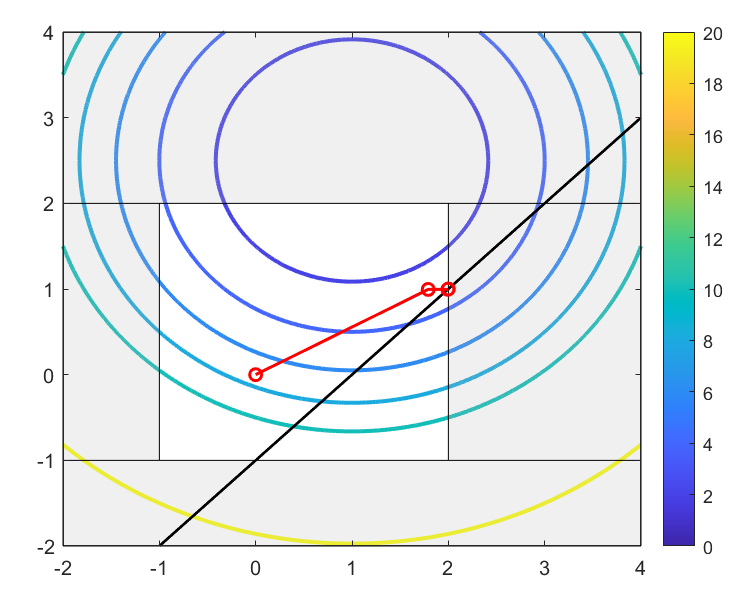
\includegraphics[scale=0.35]{figures/QP_IP_1_D.PNG}
}
\caption{ Iterative trajectory in contour of problem1}

\end{figure}
It can be seen that in the test of Problem 1, the four starting  points all reached the minimum point under the equality and inequality constraints with a small number of iterations.\\
Then the iterative trajectory in the contour for the problem2 is showed 
\vspace{-0.3cm}
\begin{figure}[H]
\centering
\setlength{\abovecaptionskip}{-0.2cm} 
\setlength{\belowcaptionskip}{-0.5cm} 
\subfigure[$A(-1,4)$]{
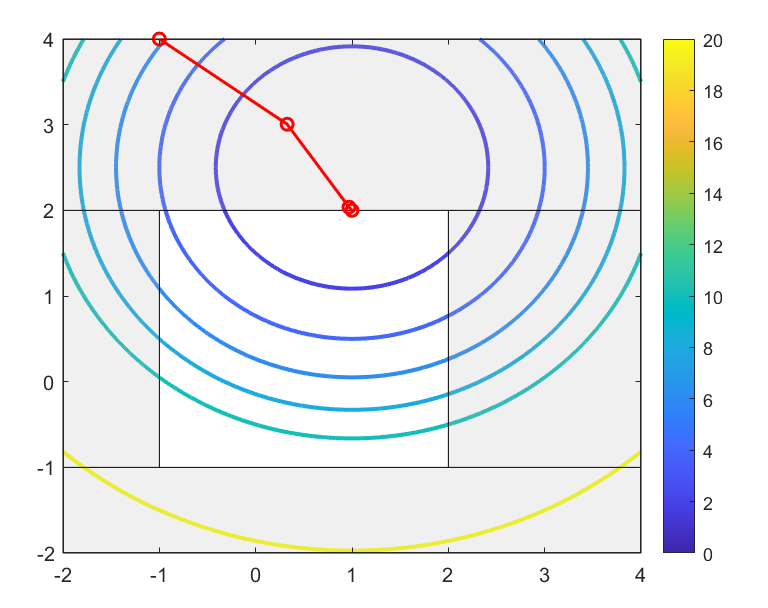
\includegraphics[scale=0.35]{figures/QP_IP_2_A.PNG}
%\caption{fig1}
}
\quad
\subfigure[$B(4,-1)$]{
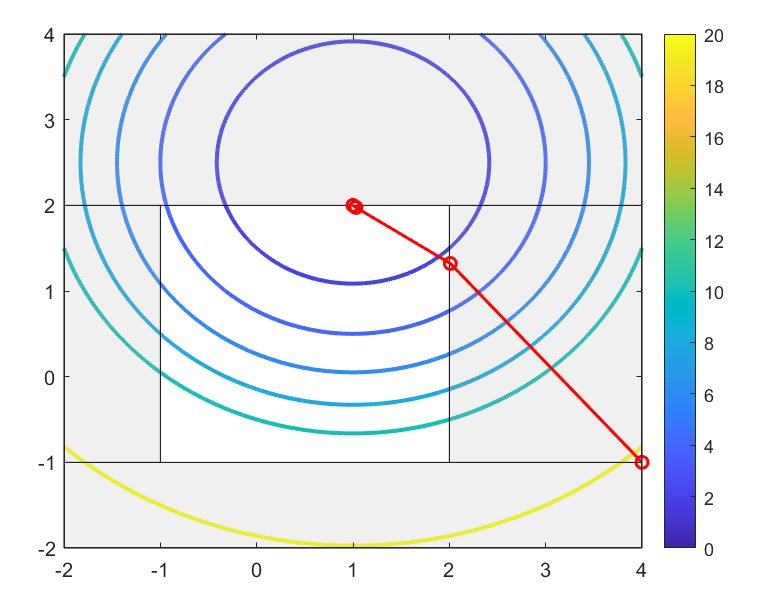
\includegraphics[scale=0.35]{figures/QP_IP_2_B.PNG}
}
\quad
\subfigure[$C(1,-1)$]{
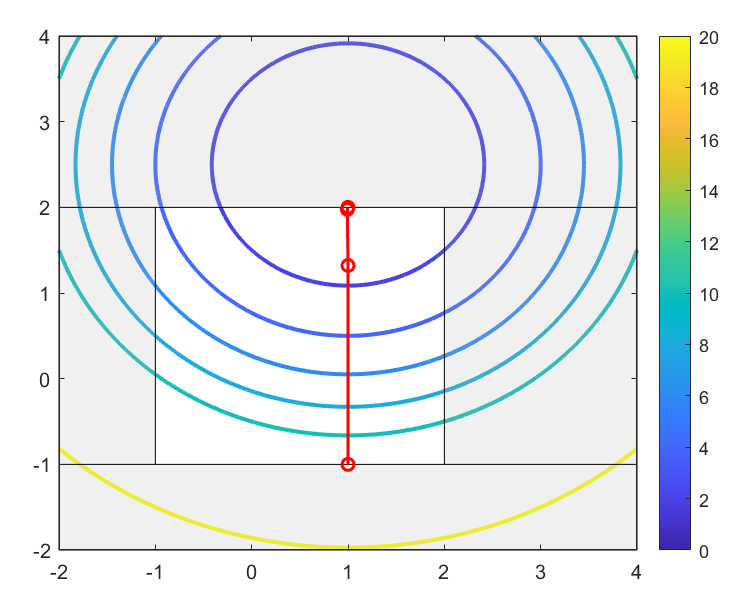
\includegraphics[scale=0.35]{figures/QP_IP_2_C.PNG}
}
\quad
\subfigure[$D(0,0)$]{
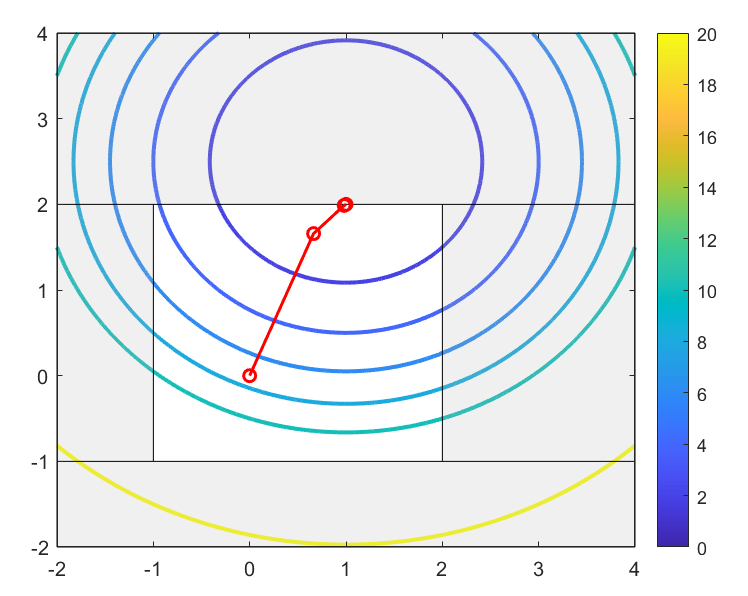
\includegraphics[scale=0.35]{figures/QP_IP_2_D.PNG}
}
\caption{ Iterative trajectory in contour of problem2}
\end{figure}

Also in the test of Problem 2, the four initial points all reached the minimum point under the constraint of inequality with a small number of iterations
%%%%%%%%%%%%%%%%%%%%%%%%%%%%%%%%%%%%%%%%%%
%%%%%%%%%%%%%%%%%%%%%%%%%%%%%%%%%%%%%%%%%%%
%%%%%%%%%%%%%%%%%%%%%%%%%%%%%%%%%%%%%%%%%%
%%%%%%%%%%%%%%%%%%%%%%%%%%%%%%%%%%%%%%%%%%%
%%%%%%%%%%%%%%%%%%%%%%%%%%%%%%%%%%%%%%%%%%
%%%%%%%%%%%%%%%%%%%%%%%%%%%%%%%%%%%%%%%%%%%
\subsection{\bfseries Primal Active-Set Algorithm}
\begin{shaded}
{Question: Write pseudo-code for a primal active-set algorithm. Explain the algorithm.}
\end{shaded}
\begin{algorithm}[H]
	\caption{Primal Active-Set Algorithm}
	\begin{algorithmic}[1]
	    \STATE Compute a feasible starting point $x_0$\\
		\STATE Let $W_0$ be the corresponding active set: $A_0=\{ i:a_i^{\prime}x_0=b_i \}$\\
		\WHILE {(not stop)}\\
		\STATE Solve a quadratic subproblem to find $p_k$\\
		\IF{($p_k=0$)}\\
		\IF{($\lambda_{i} \geq 0, \forall i \in W_{k} \cap I$)}\\
		\STATE The optimal solution has been found\\
		\STATE break\\
		\ELSE\\
		\STATE Let $j \in W_k$ be an index such that $\lambda_i<0$, Remove constraint $j$ from the working set. $W_{k+1}=W_k \backslash \{j\}$\\
		\ENDIF\\
		\ELSE\\
		\STATE Compute the distance $\alpha$ to the nearest inactive constraint in the search direction\\
		\IF{($\alpha < 1$)}\\
		\STATE $x_{k+1}=x_k+\alpha p_K$, add constraint $j$ to the working set. $W_{k+1}=W_k \cap \{ j \}$\\
		\ELSE\\
		\STATE $x_{k+1}=x_k+ p_K$, $W_{k+1}=W_k$\\
		\ENDIF\\
		\ENDIF\\
		\ENDWHILE
    \end{algorithmic}
\end{algorithm}

Similar to the characteristics of the simplex method of linear programming, both the Active-set method and the simplex method are to iterate the point and follow the constraint boundary until the optimal solution is reached. But Active-set methods form QP differ from the simplex method in that the iterates(and the solution $x^*$) are not necessarily vertices of the feasible region.\\[0.3cm]
In the first step, a set of feasible starting point needs to be computed. Here a "Phase I" method \cite{NoceWrig06} is introduced for active set algorithm. Given $\tilde{x}$ of the vector $x$, the following feasibility linear program is defined
$$\begin{array}{ll}
\min _{x, z} \quad e^{T} z \\
\text {s.t.} \qquad a_{I}^{T} x+\gamma_{i} z_{i}=b_{i} & i \in \mathcal{E} \\
\qquad  \quad a_{I}^{T} x+\gamma_{i} z_{i} \geq b_{i} & i \in \mathcal{I} \\
\qquad \quad x \in X & \\
\qquad \quad z \geq 0
\end{array}\eqno{(2.23)}$$
Where $e=(1,1,...,1)^T$, $\gamma_i=-sign\left(a_i^T\tilde{x}-b_i\right)$ for $i\in\mathcal{E} $,and $\gamma_i=1$ for $i\in\mathcal{I} $. If the initial guess is feasible then the solution to the above problem will be $(\tilde{x}, 0)$.
Primal active-set methods find a step from one iterate to the next by solving a quadratic subproblem as stated in step 2 in which some of the inequality constraints, and all the equality constraints, are imposed as equalities. This subset is referred to as the working set and is denoted at the $k$th iterate $x_k$ by $W_k$.
One important thing that need to be satisfied is the strict linear independent property of the gradients $a_i$ of the constraints in the working set $W$.
As the starting point computed, in order to check whether $x_k$ minimizes the quadratic $\phi$ in the subspace defined by the working set $W_k$, A step $p$ needs to be computed by solving an equality-constrained QP sub-problem in which the constraints corresponding
to the working set $W_k$ are regarded as equalities and all other constraints are temporarily disregarded.\\
\begin{align*}
&\min _{p}\quad \frac{1}{2} p^{\prime} G p+\left(G x_{k}+g\right)^{\prime} p \tag{2.24}\\
&s.t. \quad a_{i}^{\prime} p=0 \quad i \in \mathcal{W}_{k}
\end{align*}
Assuming that the optimal $p_k$ is nonzero, it is necessary to decide how far to move along this direction. If $x_k + p_k$ is feasible for all the constraints of the original problem, then $\alpha_k = 1$, otherwise $\alpha_k$ is a positive number less than 1. The step length $\alpha$ is defined and a new iterate is obtained
$$x_{k+1}=x_k+\alpha_kp_k\eqno{(2.25)}$$
Regarding the calculation of the step size $\alpha_k$,  the calculation of the step size is mainly to ensure that the new iteration point does not violate the constraints of the original problem. Since the constraints $i \in W_k$ are satisfied, the constraints that are not in the work set are only focused. The first step is to judge the sign of $a_i^{T}p_k$. If $a_i^{T}p_k>0$, then the analysis shows that as long as the step size $\alpha>0$0, the constraint must be satisfied, so the main concerns needed to pay attention to are those constraints with $a_i^{T}p_k<0$.\\
$$\alpha_{k}=\min \left(1, \min _{i \notin \mathcal{W}_{k}, a_{i} T_{k}<0} \frac{b_{i}-a_{i}^{T} x_{k}}{a_{i}^{T} p_{k}}\right)\eqno{(2.26)}$$
 Through the above method,the effective constraints can be continued to add to the working set until it is found that the current iteration point is the optimal solution of the current working set in a certain iteration, that is $p_k=0$ calculated at this time. Next step is to verify whether the current iteration point is the optimal solution of the original problem. The method of verification is to determine whether the Lagrange multipliers $\lambda$ corresponding to the constraints in the working set are all greater than or equal to 0. If so, the iteration is exited and the optimal solution of the original problem is given.\\
 $$\sum_{i \in \hat{w}} a_{i} \hat{\lambda}_{i}=g=G \hat{x}+c\eqno{(2.27)}$$
 If there are one or more calculated $\hat{\lambda}_{i}<0$. Then it shows that by removing one or more constraints of the working set, the value of the objective function can be further reduced. Therefore, one of the constraints with the corresponding $\hat{\lambda}_{i}<0$ will be selected, and removed from the working set $W_k$ to construct a new working set $W_{k+1}$. If there is more than one optional constraint, the constraint corresponding to the minimum (maximum absolute value) of $\hat{\lambda}_{i}$ will be removed.
 \newpage
 %%%%%%%%%%%%%%%%%%%%%%%%%%%%%%%%%%%%%%%%%%%%%%%%%%%%%%%%%%%%%%%%%%%%%%%%%%%%%%%%%%%%%%%%%%%%%%%%%%%%%%%%%%%%%%%%%%%%%%%%%%%%%%%%%%%%%%%%%%%%%%%%%%%%%%%%%%%%%%%%%%%%%%%%%%%%%%%%%%%%%%%%%%%%%%%%%%%%%%%%%%%%%%%%%%%%%%%%%%%%%%%%%%%%%%%%%%%%%%%%%%%%%%%%%%%%%%%%%%%%%%%%
 \subsection{\bfseries Primal Active-Set Algorithm implementation}
\begin{shaded}
{Question: Implement the primal active-set algorithm and test it. You must provide commented code as well as driver files to test your code, documentation that it works,
and performance statistics}
\end{shaded}

The main matlab code of Primal Active-Set Algorithm is showed here, and the function "As\_sub" which solve the sub-problem is stated in appendix \ref{6.2.3}.

{\setmainfont{Courier New Bold} \scriptsize            
\begin{lstlisting}
function [x,lam,exitflag,output]=Pri_AsQp(H,g,Ae,be,Ai,bi,x0)
% Pri_AsQp   Primal Active-Set Algorithm
%
%          min  0.5*H'*x*H+g'*x
%           x
%          s.t. Ae x  = be      
%               Ai x >= bi      
%
% Syntax: [x,lam,exitflag,output]=Pri_AsQp(H,g,Ae,be,Ai,bi,x0)
%         output.lam: Lagrange multiplier
%         output.x_plot: Iteration trajectory              
%Initialization
%Ax>=b;
epsilon=1.0e-9;
err=1.0e-6;
iteration=0;
x=x0;
n=length(x);
iteration_max=20;
ne=length(be);
ni=length(bi);
lam=zeros(ne+ni,1);
index=ones(ni,1);
output.x_plot=[x0'];
output.lam=[lam'];

%initialize the active set(index=1)
for(i=1:ni)
    if(Ai(i,:)*x>bi(i)+epsilon)
        index(i)=0;
    end
end
%main program
while(iteration<=iteration_max)
    
    Aee=[];
% if the start point x is on the Equality Constraint or on the edge of the
% Equality Constraint, put it in active set.
    if(ne>0)
        Aee=Ae;
    end
    for j=1:ni
        if(index(j)>0)
            Aee=[Aee;Ai(j,:)];
        end
    end
    %Solve subproblem to find p and Compute Lagrange multipliers
    gk=H*x+g;
    [m1,n1]=size(Aee);
    [p,lam]=As_sub(H,gk,Aee,zeros(m1,1));
    if(norm(p)<=err)
        lambda_min=0.0;
        if(length(lam)>ne)
            [lambda_min,jk]=min(lam(ne+1:end));
        end
        if(lambda_min>=0)
            exitflag=1;
        else
            exitflag=0;
            %remove the (Lagrange multipliers min) inequlity Constraint
            %form active set
            for(i=1:ni)
                if(index(i)&(sum(index(1:i)))==jk)
                    index(i)=0;
                    break;
                end
            end
        end
        iteration=iteration+1;
    else
        exitflag=0;
        %computer the step length
        alpha=1.0;
        tm=1.0;
        for(i=1:ni)
            if((index(i)==0)&(Ai(i,:)*p<0))
                tm1=(bi(i)-Ai(i,:)*x)/(Ai(i,:)*p);
                if(tm1<tm)
                    tm=tm1;
                    ti=i;
                end
            end
        end
        
        alpha=min(alpha,tm);
        x=x+alpha*p;
        %update the active set
        if(tm<1)
            index(ti)=1;
        end
    end
    if(exitflag==1)
        break;
    end
    iteration=iteration+1;
    output.x_plot=[output.x_plot;x'];
    if(length(lam)<(ne+ni))
        lam=[lam;zeros(ne+ni-length(lam),1)];
    end
    output.lam=[output.lam;lam'];
end
output.fval=0.5*x'*H*x+g'*x;
output.iter=iteration;
\end{lstlisting}}
In the later chapter on the comparison of the two algorithms, an algorithm with a test problem that can be randomly generated and control the size of the variable will be test. Here is just a simple verification of the feasibility of the algorithm.\\
The same two problems tested by Primal-dual interior-point algorithm in section 2.4 are used. However, the different starting points for active-set algorithm should be chose because the iteration of active-set method can only be implemented in the feasible region. And for quadratic problem which has equality constraints, the starting points have to be located at the equality constraints. So we choose starting points $A_1(0,-1)$ and $B_1(1,0)$ for the problem2, and starting points $A_2(0,-1)$, $B_2(2,0)$, $C_2(0,2)$ and $D_2(-1,0)$ for the problem2.\\[0.3cm]
The driver files are stated in the appendix \ref{6.2.4} and \ref{6.2.5}. The iterative trajectory in the contour for the problem1 is showed here
\begin{figure}[H]
\centering
\subfigure[$A(0,-1)$]{
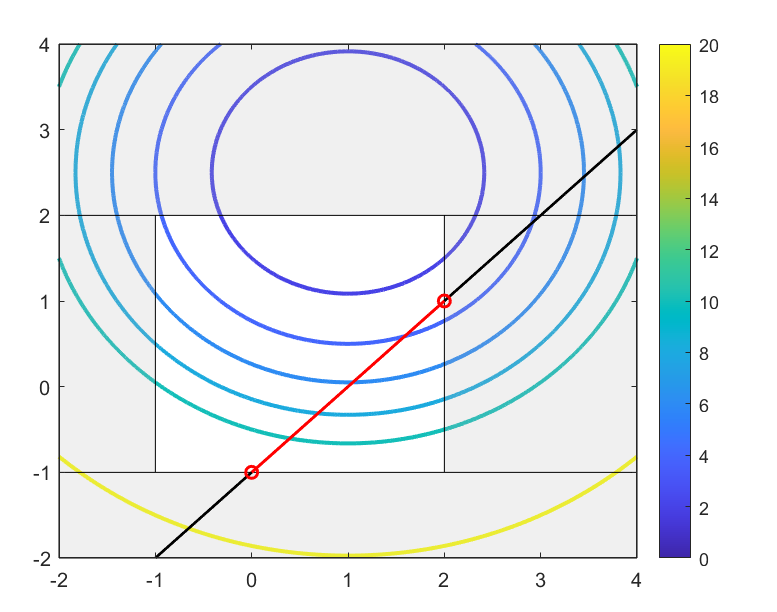
\includegraphics[scale=0.4]{figures/QP_AS_1_A.PNG}
%\caption{fig1}
}
\quad
\subfigure[$B(1,0)$]{
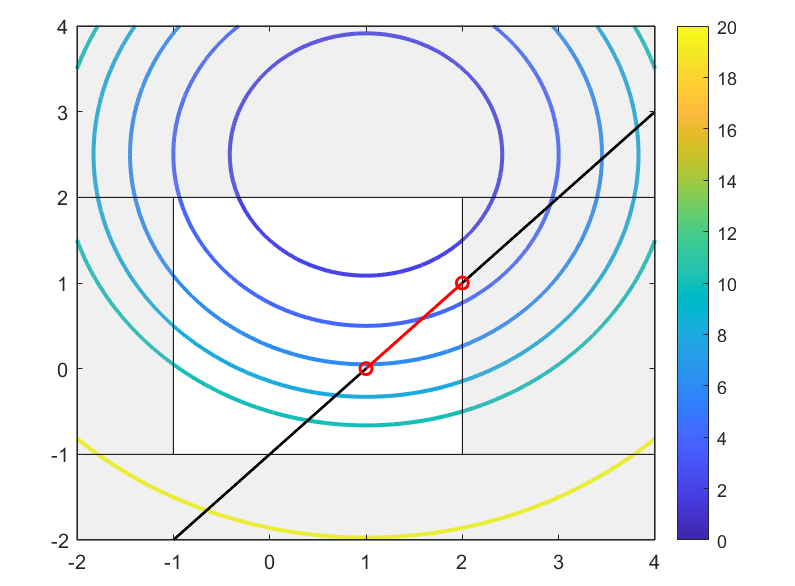
\includegraphics[scale=0.4]{figures/QP_AS_1_B.PNG}
}
\caption{ Iterative trajectory in contour of problem1}
\end{figure}
It can be seen that in the test of Problem 1, the two starting  points all reached the minimum point under the equality and inequality constraints with a small number of iterations.\\
Then the iterative trajectory in the contour for the problem2 is showed 
\begin{figure}[H]
\centering
\subfigure[$A(0,-1)$]{
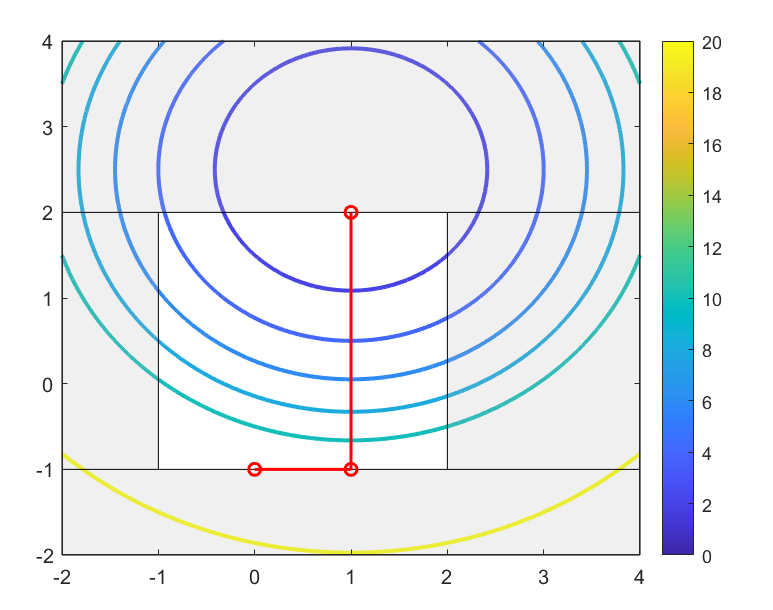
\includegraphics[scale=0.4]{figures/QP_AS_2_A.PNG}
%\caption{fig1}
}
\quad
\subfigure[$B(2,0)$]{
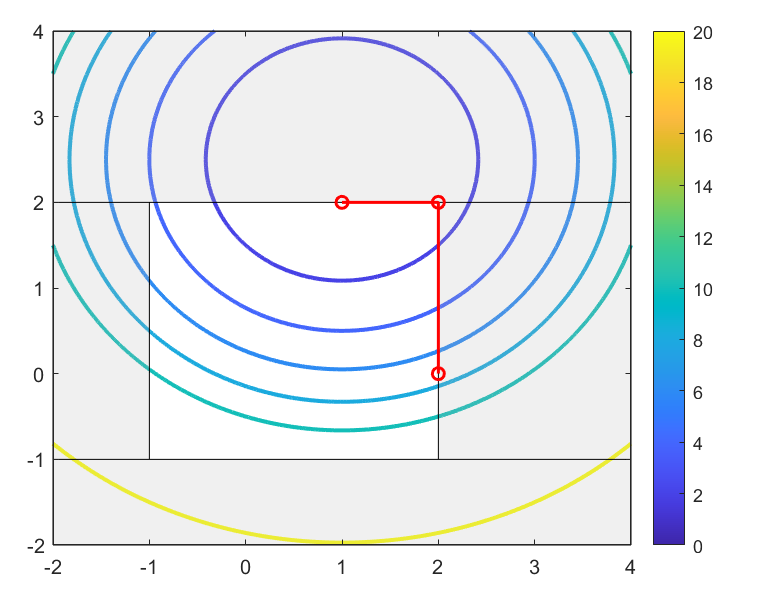
\includegraphics[scale=0.4]{figures/QP_AS_2_B.PNG}
}
\quad
\subfigure[$C(0,2)$]{
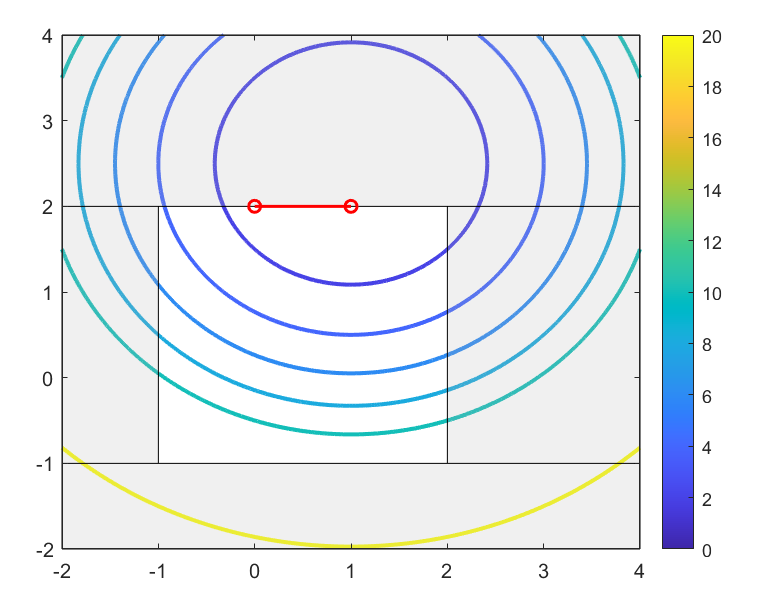
\includegraphics[scale=0.4]{figures/QP_AS_2_C.PNG}
}
\quad
\subfigure[$D(-1,0)$]{
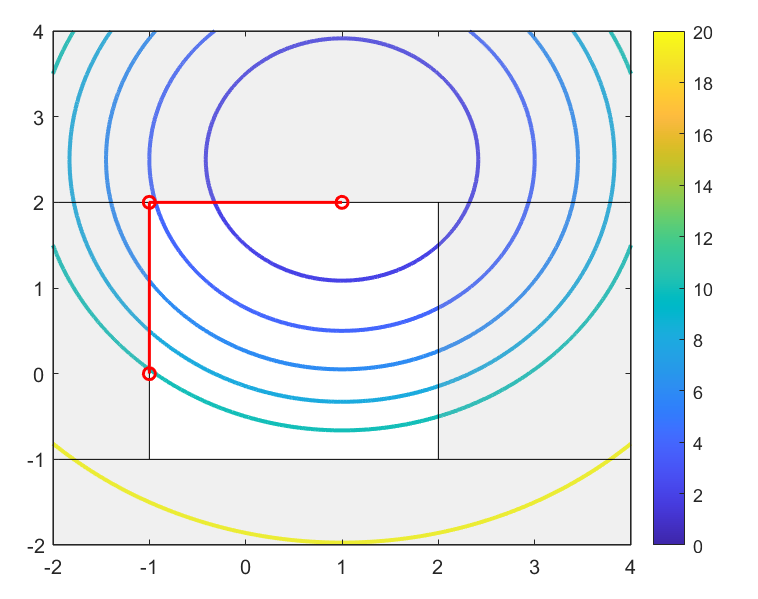
\includegraphics[scale=0.4]{figures/QP_AS_2_D.PNG}
}
\caption{ Iterative trajectory in contour of problem2}
\end{figure}

Also in the test of question 2, the four initial points all reached the minimum point under the constraint of inequality with a small number of iterations.
%%%%%%%%%%%%%%%%%%%%%%%%%%%%%%%%%%%%%%%%%%%%%%%%%%%%%%%%%%%%%%%%%%%%%%%%%%%%%%%%%%%%%%%%%%%%%%%%%%%%%%%%%%%%%%%%%%%%%%%%%%%%%%%%%%%%%%%%%%%%%%%%%%%%%%%%%%%%%%%%%%%%%%%%%%%%%%%%%%%%%%%%%%%%%%%%
\newpage
\subsection{\bfseries Comparison of algorithms}
\begin{shaded}
{Question: Compare the performance of your primal-dual interior-point algorithm, primal
active-set algorithm, and quadprog of Matlab (or equivalent QP library functions). Provide scripts that demonstrate how you compare the software and comment on the tests and the results.}
\end{shaded}
In order to better test the performance of the algorithm, a test problem that can randomly generate parameters and adjust the number and size of variables is designed.
\begin{align*}
&\min_{x} \quad \phi=\frac{1}{2} x^{\prime} H x+g^{\prime} x \qquad H\in \mathbb{R}^{n \times n} \quad g\in \mathbb{R}^{n \times 1} \tag{2.28}\label{con:op2.28}\\
& s.t. \quad A^{\prime}x=b \qquad \qquad \qquad A\in \mathbb{R}^{n \times m}\\
& \quad \quad  0\le x \le 10
\end{align*}
From the optimality conditions, it is  defined that
\begin{align*}
&x_{i}=\left\{\begin{array}{ll}
\text { random positive number } & i=1,2, \ldots, m \\
0 & i=m+1, m+2, \ldots, n
\end{array}\right \tag{2.29}\\
& z_{i}=\left\{\begin{array}{ll}
\text { random positive number } & i=m+1, m+2, \ldots, n \\
0 & i=1,2, \ldots, m
\end{array}\right \tag{2.30}\\
& y=\text{random vector}\\
& \nabla_{x} L\left(x,y,z\right)=Hx+g-Ay-z=0 \Leftrightarrow g=Ay+z-Hx\tag{2.31}\\
& \nabla_{y} L\left(x,y,z\right)=-\left(A^{\prime}x-b\right)=0 \Leftrightarrow b=A^{\prime}x\tag{2.32}\\
\end{align*}
Where the positive definite Hessian $H$ is designed by $H=P^{\prime}HP+Q, \quad P\in \mathbb{R}^{n \times n}, Q\in \mathbb{R}^{n \times n}$, The $P$ matrix is random positive matrix and $Q$ is an identity matrix.
In order to compare the performance of these two algorithms and quadprog, first the same initial feasible point solved by the method stated in active-set method(Here the "dual simplex method" in linprog is used) is used for three algorithms. And the iteration numbers and deviation expressed by $\left\|x^*-x_{result}\right\|_2$($x^*$ is the correct optimal solution and $x_{result}$ is the optimal solution obtained by the prim-dual interior point method) is showed to analyze the performance. Here the number of variables($n$) is adjusted from $10-200$ Please see the driver files in the appendix \ref{6.2.6}.
\begin{figure}[H]
\centering
\setlength{\abovecaptionskip}{-0.2cm} 
\setlength{\belowcaptionskip}{-0.5cm} 
\subfigure[Deviation]{
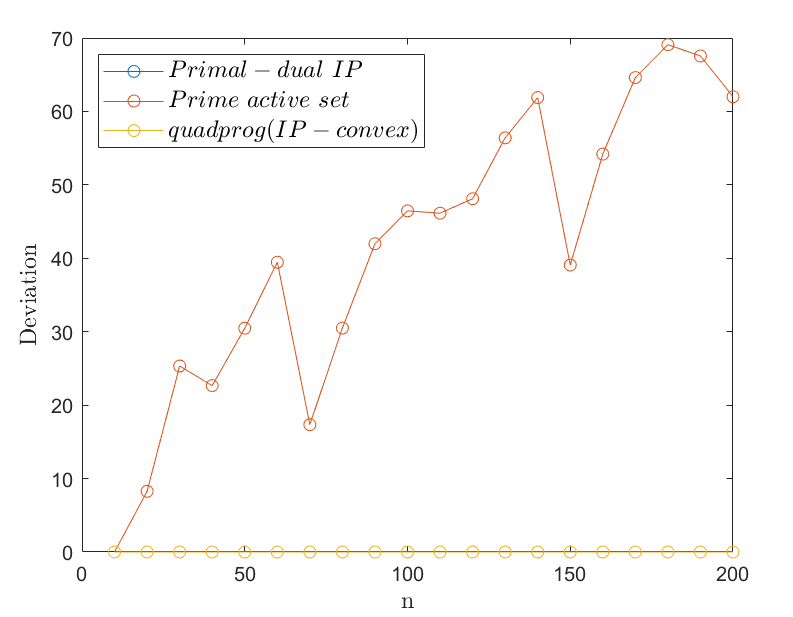
\includegraphics[scale=0.5]{figures/QP_ACCURACY.PNG}
%\caption{fig1}
}
\quad
\subfigure[Iteration numbers]{
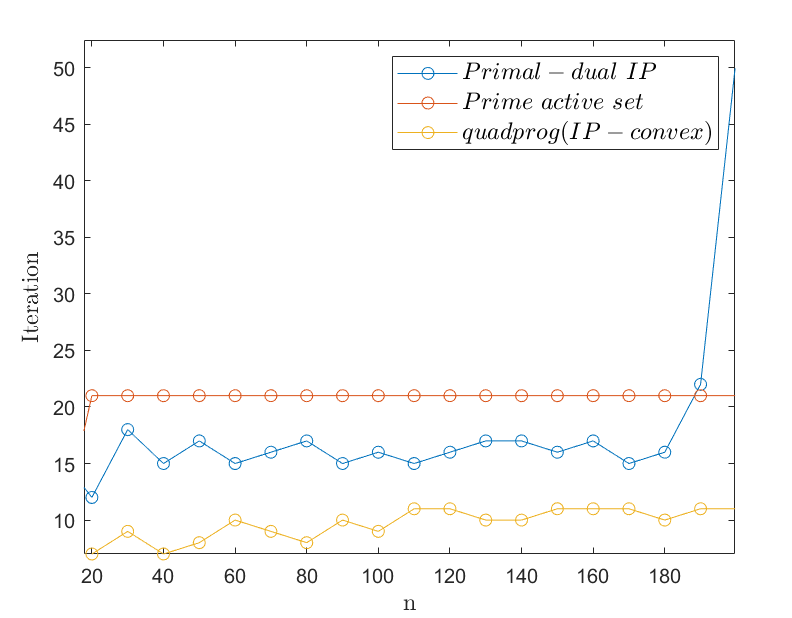
\includegraphics[scale=0.5]{figures/QP_ITERATION.PNG}
}
\caption{Performance of prime-dual interior-point algorithm, primal
active-set algorithm, and quadprog}
\end{figure}
First of all, for the deviation curve obtained by the three algorithms, it should be noted that the deviation curve obtained by the interior point method used by quadprog is exactly the same as the deviation curve of the prime-dual interior point method implemented by ourselves, so only two curves are displayed. It can be seen that as the number of variables increases, the deviation of the active set method gradually becomes larger, and the deviation of the obtained result from the correct value obtained by either the interior point method implemented or the interior point method using quadprog can be kept at a small value all the time, and does not increase with the increase of the number of variables.\\

Then for the curve of the number of iterations obtained by the three algorithms, it first can be seen that no matter how the number of variables increases, the interior point method of quadprog has been kept at a small number of iterations. It can be seen that when the number of variables is less than 180($n<180$), Although the number of iterations of the interior point method implemented is smaller than that of the active set method, when the number of variables is greater than 180($n>180$) , the number of iterations of the interior point method suddenly jumps more than the number of iterations of the active set method, and the iteration of the active set method has been stable at about 20 times, and does not change with the increase of the number of variables. It can be inferred that the reason for this difference may be 1. The stopping criteria set by the interior point method implemented and the quadprog interior point method are different 2. The starting point of the interior point method implemented and the interior point method of quadprog is the starting point calculated by the active set method, which may affect the number of iterations.

%%%%%%%%%%%%%%%%%%%%%%%%%%%%%%%%%%%%%%%%%%%%%%%%%%%%%%%%%%%%%%%%%%%%%%%%%%%%%%%%%%%%%%%%%%%%%%%%%%%%%%%%%%%%%%%%%%%%%%%%%%%%%%%%%%%%%%%%%%%%%%%%%%%%%%%%%%%%%%%%%%%%%%%%%%%%%%%%%%%%%%%%%%%%%%%%%%%%%%%%%%%%%%%%%%%%%%%%%%%%%%%%%%%%%%%%%%%%%%%%%%%%%%%%%%%%%%%%%%%%%%%%
 \subsection{\bfseries Markowitz’ portfolio optimization problem as QP}
\begin{shaded}
{Question: Demonstrate that Markowitz’ portfolio optimization problem can be expressed as
a QP in the form and test the primal-dual interior-point QP algorithm, the
primal active-set QP algorithm, and the library QP algorithm e.g. quadprog}
\end{shaded}
Consider a financial market with 5 securities.\\[0.3cm]
\begin{tabular}{c|ccccc|c}
\hline Security & \multicolumn{5}{|c|} { Covariance } &  Return\\
\hline 1 & 2.30 & 0.93 & 0.62 & 0.74 & -0.23 & 15.10 \\
2 & 0.93 & 1.40 & 0.22 & 0.56 & 0.26 & 12.50 \\
3 & 0.62 & 0.22 & 1.80 & 0.78 & -0.27 & 14.70 \\
4 & 0.74 & 0.56 & 0.78 & 3.40 & -0.56 & 9.02 \\
5 & -0.23 & 0.26 & -0.27 & -0.56 & 2.60 & 17.68 \\
\hline
\end{tabular}\\[0.3cm]
The quadratic programming form of Markowitz’ portfolio optimization problem
\begin{align*}
&\min_{x \in \mathcal{R}^n} \quad \phi=\frac{1}{2}x^{\prime}Hx \tag{2.33}\\
& s.t. \quad \mu^{\prime}x= R\\
& \quad \quad \sum_{i=1}^{n}x_i=1\\
& \quad \quad \ x \ge 0
\end{align*}
Then a portfolio with return, $R = 10.0$ is computed, to obtain minimal risk and the optimal
portfolio, by the primal-dual interior-point QP algorithm, the
primal active-set QP algorithm, and the "quadprog"(The interior-point-convex is used here). Please see the driver files in appendix \ref{6.2.7}. The result and the iteration numbers are showed\\
The primal-dual interior-point QP algorithm
\begin{align*}
&    x=(0,0.2816,0,0.7184,0)^{\prime}\\
&Return: \quad E\{ R\}=10\\
&Risk(Variance):\quad V\{ R\}=x^{\prime}Hx=2.0923\\
&Iteration=6
\end{align*}
The
primal active-set QP algorithm
\begin{align*}
&    x=(0,0.2816,0,0.7184,0)^{\prime}\\
&Return: \quad E\{ R\}=10\\
&Risk(Variance):\quad V\{ R\}=x^{\prime}Hx=2.0923\\
&Iteration=4
\end{align*}
The "quadprog" with "interior-point-convex"
\begin{align*}
&    x=(0,0.2816,0,0.7184,0)^{\prime}\\
&Return: \quad E\{ R\}=10\\
&Risk(Variance):\quad V\{ R\}=x^{\prime}Hx=2.0923\\
&Iteration=5
\end{align*}